% při kompilaci dokumentu LuaLaTeXem dojde k chybě, protože
% nedefinuje \pdfpagewidth a \pdfpageheight. 
% Balíček luatex85 to napravuje
\ifdefined\directlua
\RequirePackage{luatex85}
\fi

\documentclass{csbulletin}
% \usepackage[T1]{fontenc}
% \usepackage[utf8]{inputenc}
\usepackage{fontspec}
\setmainfont[Ligatures={TeX,Rare}]{Latin Modern Roman}
\selectlanguage{czech}
\usepackage{luavlna}
\usepackage[noautomatic]{responsive}
\usepackage{lua-widow-control}
\usepackage{csquotes}
\usepackage{linebreaker}
\usepackage{amsmath,amsfonts}

\usepackage{graphicx}
\usepackage{caption}
\usepackage{subcaption}
\usepackage{lipsum}


\usepackage[
  backend=biber,
  style=iso-numeric,
  sortlocale=cs,
  autolang=other,
  bibencoding=UTF8,
  mincitenames=2,
  maxcitenames=2,
]{biblatex}
\addbibresource{responsive.bib}
\usepackage[
  implicit=false,
  hidelinks,
]{hyperref}


\newcommand\balicek[1]{\textit{#1}}
\newcommand\program[1]{#1}

% pro případ, kdy je \lipsum moc velké 
\newcommand\smalllipsum{%
Lorem ipsum dolor sit amet,
consectetuer adipiscing elit.
Ut purus elit, vestibulum ut,
placerat ac, adipiscing vitae,
felis. Curabitur dictum gravida 
mauris. Nam arcu libero, nonummy 
eget, consectetuer id, vulputate 
a, magna. Donec vehicula augue eu neque.
}

\newcommand\printsize[1]{\csname #1\endcsname\par\noindent Sample\par}
\newcommand\showscale[2][.5\textwidth]{%
      % \setsizes[38]{25}
      \printsize{huge}
      \printsize{LARGE}
      \printsize{Large}
      \printsize{large}
      \hrule
      \printsize{normalsize}
      \hrule
      \printsize{small}
      \printsize{footnotesize}
}


\begin{document}

\title{Responzivní design a automatická sazba s Lua\LaTeX em}
\EnglishTitle{Responsive Design and Automatic Typesetting with Lua\LaTeX}
\author{Michal Hoftich}
\podpis{Michal Hoftich, \url{michal.h21@gmail.com}}
\maketitle

\begin{abstract}
Tento článek se zaměřuje na použití metod responzivního designu pro zobrazení
webových stránek na zařízeních s různou velikostí displejů, jako jsou mobilní
telefony, tablety, velké monitory a tiskárny. Tyto metody umožňují optimalizaci
čitelnosti dokumentu na všech zařízeních pomocí použití různých velikostí
písma, jednotlivých prvků na stránce a okrajů.

Představíme způsob, jak lze podobné funkcionality dosáhnout
pomocí \LaTeX u. Konkrétně se zaměřuje na využití Lua\LaTeX u pro automatizovanou
sazbu s pomocí balíčků \balicek{Responsive}\cite{responsive} pro nastavení velikosti písma a řádkového prokladu
podle velikosti stránky, \balicek{Luavlna} \cite{luavlna} pro zamezení výskytu jednopísmenných předložek
na koncích řádků, \balicek{Lua-widow-control}  \cite{lua-widow-control} pro omezení osamocených řádků na koncích a
začátcích stránek a \balicek{Linebreaker} \cite{linebreaker}, který brání přetečení řádků.

Díky těmto metodám lze použít jeden zdrojový dokument pro různé výstupy, jako
jsou tiskové verze, čtečky e-knih a webové stránky, a dosáhnout optimálního
zobrazení dokumentu na všech zařízeních.
\end{abstract}
\klicovaslova: automatická sazba, responzivní design, Lua\LaTeX


\section{Úvod}

Před časem jsem si pořídil čtečku elektronických knih, ale i přesto většinu
textů čtu z obrazovky svého PC, protože pochází z webových zdrojů, především 
různých blogů. To má za důsledek několik problémů, například únavu očí, bolesti zad
z příliš dlouhého sezení na židli, nemluvě o zbytečně spotřebované elektrické
energii. Napadlo mě tedy, že bych bych si delší články ukládal pro pozdější
přečtení na čtečce. K tomuto účelu samozřejmě existuje řada aplikací, ale 
já se rozhodl vytvořit si vlastní, kterou si přizpůsobím přesně svým potřebám
a preferencím. Další motivací je možnost naučit se něco nového a vytvořit
balíčky, které budou užitečné i pro další uživatele \TeX u. 

Protože díky Lua\TeX u je v \TeX ových distribucích dostupný programovací jazyk 
Lua, využil jsem ho pro vytvoření svého projektu \program{Rmodepdf} \cite{rmodepdf}.
Ten využívá balíček \balicek{LuaXML} \cite{luaxml} pro 
transformaci HTML na \TeX{} a příkazy \program{Curl} pro stažení stránky, \program{Tidy} 
pro opravu chyb v HTML a \program{Rdrview} \cite{rdrview}, který odstraní
ze stránky navigační prvky, reklamy a jiné rušivé elementy. \program{Rdrview} 
tak funguje podobně jako mód zobrazení čtečky v prohlížeči \program{Firefox}
(ilustrováno v obrázku~\ref{fig:readermode}).

V následujícím textu se však nezaměřím na samotný \program{Rmodepdf}.
Myslím, že pro čtenáře bude užitečnější popis metod pro automatickou sazbu,
které lze využít i pro jiné účely, například při konverzi z dokumentů ve formátu MS Word, 
nebo elektronických knih ve formátu Epub. Zde nevyužijeme funkci
odstraňování navigačních prvků ze stránky, ale můžeme zde využít
přizpůsobení velikosti písma velikosti stránky nebo automatické řešení
typografických problémů či špatně zalomených řádků.

\begin{figure}[tbp]

  \centering
  \caption{Ukázka použití režimu \emph{zobrazení čtečky} v prohlížeči \program{Firefox}}
  \label{fig:readermode}

  \begin{subfigure}[t]{0.45\textwidth}
    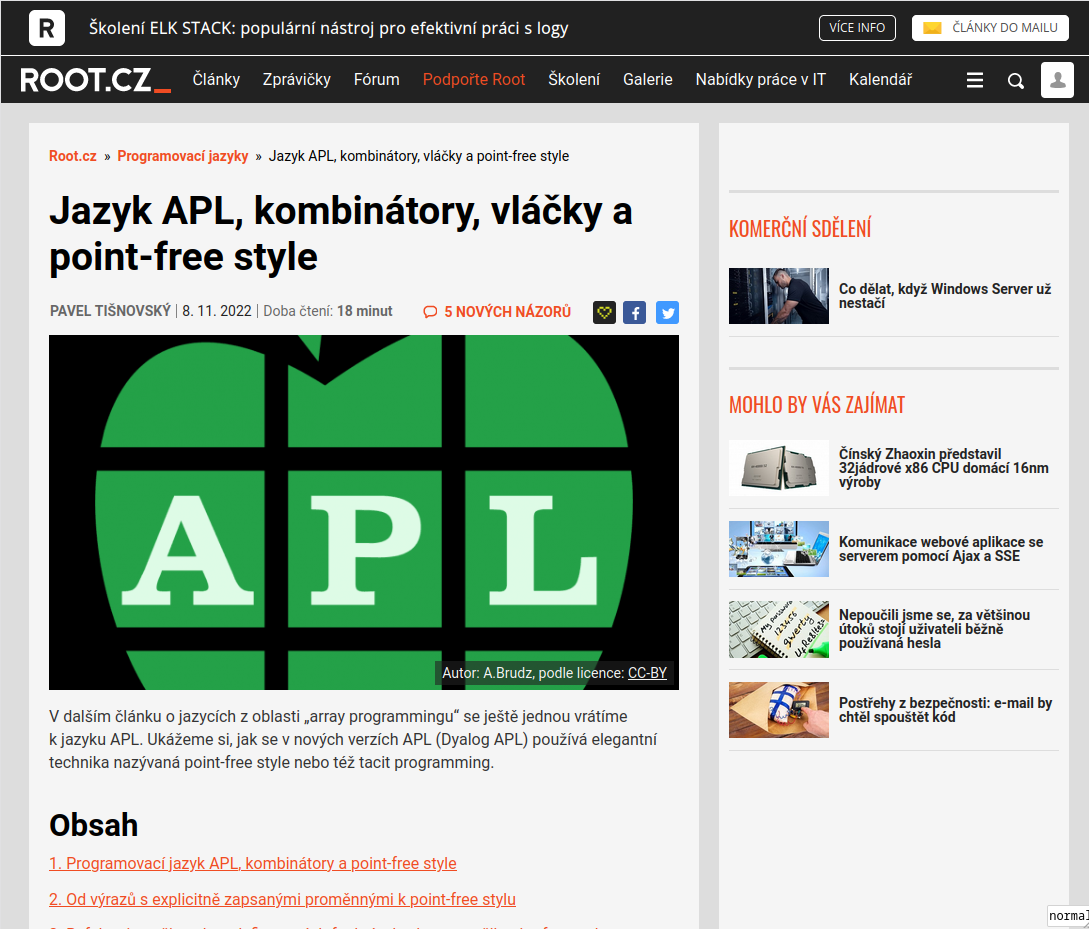
\includegraphics[width=\textwidth]{img/root-balast.png}
    \caption{Stránka s ovládacími prvky a reklamami}
  \end{subfigure}
  \hfill
  \begin{subfigure}[t]{0.45\textwidth}
    \includegraphics[width=\textwidth]{img/root-čtečka.png}
    \caption{Stránka v zobrazení čtečky}
  \end{subfigure}
\end{figure}

% \section{Jak s pomocí \LaTeX u převést webovou stránku na PDF}

% % https://github.com/eafer/rdrview

% \begin{verbatim}
% $ rdrview -H <url> | pandoc -f html -t latex -V lang=cs \
%   --template template.tex output.html > output.tex
% \end{verbatim}

\section{Responzivní design}

Prvním problémem, který jsem řešil, bylo nastavení správné velikosti písma 
z hlediska čitelnosti. 
Výchozí velikost písma v \LaTeX u je 10 bodů, bez ohledu na velikost
stránky. To je vhodná velikost pro stránku formátu A5. Pro formát
A4 by měla být větší, naopak pro menší displeje čteček a mobilních
telefonů může být menší. Stejný problém řeší webové prohlížeče,
které musí zobrazit text jak na velkých monitorech PC, tak na
menších displejích notebooků, tabletů a mobilních telefonů. 
Řešením, který používají, je \textit{responzivní design}.



Responzivní design je způsob návrhu webových stránek, který umožňuje
pružné a dynamické přizpůsobení vzhledu a uspořádání obsahu stránky
různým zobrazovacím zařízením. Jedním z klíčových prvků responzivního
designu je flexibilní struktura, která umožňuje přizpůsobit velikost
prvků na stránce zobrazovacímu zařízení.

Dalším důležitým prvkem jsou media queries, které umožňují definovat
pravidla, která se aplikují na základě vlastností zobrazovacího
zařízení, jako je velikost displeje, druh displeje, atd. Díky těmto
vlastnostem může stejný kód stránky být dobře zobrazen jak na velkém
monitoru, tak na mobilních zařízeních. Ukázku reálného využití 
můžete vidět na obrázku~\ref{fig:responzivni}.


\begin{figure}[tbp]
  \caption{Ukázka zobrazení webové stránky s využitím responzivního designu}
  \label{fig:responzivni}
\begin{subfigure}[t]{0.74\textwidth}
    
\includegraphics[width=\textwidth]{img/pedf-web-big.png}
    \caption{Ukázka stránky na velkém monitoru}
\end{subfigure}
\hfill
\begin{subfigure}[t]{0.24\textwidth}
    \includegraphics[width=\textwidth]{img/pedf-web-small.png}
    \caption{Ukázka stránky na malém displeji}
\end{subfigure}
\end{figure}

Můj nový balíček \balicek{Responsive} \cite{responsive} se těmito zásadami inspiroval. 
Jeho hlavní funkcí je nastavení velikosti písma podle velikosti stránky
a přibližného počtu znaků, které by se měly vejít na stránku. 
Dále nastavuje typografickou stupnici (ovlivňuje velikost písma například 
u nadpisů nebo poznámek pod čarou), písmovou osnovu a podporuje
jednoduchou verzi media queries.

\subsection{Nastavení balíčku \balicek{Responsive}}

\balicek{Responsive} automaticky nastavuje velikost písma, řádkový proklad
a typografickou stupnici na začátku dokumentu. Výchozí hodnoty můžeme změnit
pomocí voleb balíčku, nebo příkazem \verb|\ResponsiveSetup|, který můžeme 
využít i v dokumentu, například pro lokální změny nastavení písma. 

Hlavní volby balíčku jsou tyto:

\begin{description}
  \item[noautomatic] – nenastavovat velikost písma automaticky na začátku dokumentu
  \item[characters] – počet znaků při automatickém nastavení velikosti písma
  \item[scale] –  typografická stupnice použitá pro velikosti řezů písma
  \item[lineratio] – poměr využitý při výpočtu řádkového prokladu
\end{description}

\subsection{Základní velikost písma}

Velikost písma můžeme nastavit pomocí příkazu \verb|\setsizes{<počet znaků na|\allowbreak\verb|řádek>}|. 
\balicek{Responsive} se snaží nastavit velikost písma tak, aby na řádku byl v průměru
požadovaný počet znaků. Skutečný počet znaků samozřejmě záleží na použitém textu, ve 
skutečnosti bývá mírně vyšší.

Pokud neuvedeme počet znaků, použije se hodnota volby \texttt{characters}.
Následující příklad využívá právě nastavení této volby. Obrázek~\ref{fig:fontsize} 
ukazuje, jak se stejný text může v daném rámci zobrazit rozdílně v závislosti na
nastavených volbách.

\begin{verbatim}
\begin{minipage}{5cm}
\ResponsiveSetup{characters=55}
\setsizes{}
\lipsum[1]
\end{minipage}}
\end{verbatim}

\begin{figure}[tbp]
  \caption{Rozdíl velikosti písma v závislosti na počtu znaků}
  \label{fig:fontsize}
  \begin{subfigure}[t]{0.45\textwidth}
\fbox{%
\begin{minipage}{5cm}
\ResponsiveSetup{characters=55}
\setsizes{}

\lipsum[1]

\end{minipage}}
\caption{\texttt{characters=55}}
\end{subfigure}
\hfill
\begin{subfigure}[t]{0.45\textwidth}
\fbox{%
\begin{minipage}{5cm}
\ResponsiveSetup{lineratio=38,characters=25}
\setsizes{}

Lorem ipsum dolor sit amet,
consectetuer adipiscing elit.
Ut purus elit, vestibulum ut,
placerat ac, adipiscing vitae,
felis. Curabitur dictum gravida 
mauris. Nam arcu libero, nonummy 
eget, consectetuer id, vulputate 
a, magna. Donec vehicula augue eu neque.

\end{minipage}}
\caption{\texttt{characters=25, lineratio=38}}
\end{subfigure}
\end{figure}

\subsection{Řádkový proklad}

V základním nastavení \LaTeX u je řádkový proklad nastavený
na velikost písma násobený hodnotou $1.2$. Pro jiná 
písma a velikosti stránky může být vhodná jiná velikost prokladu.
Stejně tak mohou být rozdílné hodnoty pro tištěnou a elektronickou 
verzi dokumentu. 

Inspiroval jsem se článkem Edoarda Cavazza \cite{cavazza} o čitelnosti
a přidal podporu pro nastavení řádkové prokladu na základě poměru výšky 
malých písmen a proměnné \texttt{lineratio}. Ten se získá následujícím 
výpočtem: 

\[\text{proklad} = \frac{1\text{ex}}{\text{lineratio}/ 100}\]

Jaký vliv mají změny hodnoty \texttt{lineratio} můžete pozorovat v obrázku~\ref{fig:lineratio}. 
Volba optimální hodnoty je individuální a pro dosažení maximální čitelnosti
výstupu je vhodné vyzkoušet několik různých hodnot a vybrat tu nejvhodnější.




\begin{figure}[tbp]
  \caption{Změna řádkového prokladu změnou hodnoty \texttt{lineratio}}
  \label{fig:lineratio}
  \begin{subfigure}[b]{0.45\textwidth}
\fbox{%
\begin{minipage}{5cm}
\ResponsiveSetup{lineratio=38}
\setsizes{65}

\lipsum[1]

\end{minipage}}
\caption{lineratio=38}
\end{subfigure}
\begin{subfigure}[b]{0.45\textwidth}
\fbox{%
\begin{minipage}{5cm}
\ResponsiveSetup{lineratio=34}
\setsizes{65}

\lipsum[1]

\end{minipage}}
\caption{lineratio=34}
\end{subfigure}
\end{figure}

\subsection{Typografická stupnice}

Typografická stupnice je soubor předem stanovených velikostí písma, které jsou
používány pro vytváření jednotného vizuálního stylu dokumentu nebo webové
stránky. Tyto velikosti jsou obvykle vyjádřeny v bodové jednotce a postupně se
zvětšují nebo zmenšují o konkrétní interval, který leží na stupnici.

Typografická stupnice může obsahovat velikosti pro nadpisy, poznámky pod čarou a běžný
text. Správné používání typografické stupnice pomáhá vytvořit vizuální
hierarchii, která zlepšuje čitelnost a estetický dojem textu. 
Více informací o typografických stupnicích naleznete v článku Spencera Mortensena
\cite{mortensen}. 

V \LaTeX u je typografická stupnice dostupná pomocí příkazů jako \verb|\large|, \verb|\Large|, \verb|\LARGE|,
\verb|\huge|, nebo třeba \verb|\scriptsize|. Každý z těchto příkazů je od předešlé velikosti 
vzdálený o jeden interval.  Výchozí stupnice v balíčku \balicek{Responsive} je nejbližší stupnici použitou v \LaTeX u.
V Mortensenově článku se nazývá \textit{tetratonická}. Balíček nabízí i další stupnice v článku popsané,
například \textit{golden}, založenou na zlatém řezu. Efekt použití stupnice je zobrazen na 
obrázku~\ref{fig:stupnice}.

\begin{figure}[tbp]
  \caption{Ukázka typografických stupnic (výchozí velikost písma je zvýrazněna linkami)}
  \label{fig:stupnice}
  \begin{subfigure}[b]{0.45\textwidth}
\fbox{%
\begin{minipage}{5cm}
\setsizes{45}

\showscale{}

\end{minipage}}
\caption{Výchozí stupnice}
\end{subfigure}
\begin{subfigure}[b]{0.45\textwidth}
\begin{verbatim}
\ResponsiveSetup{scale=golden}
\end{verbatim}
\fbox{%
\begin{minipage}{5cm}
\ResponsiveSetup{scale=golden}
\setsizes{45}

\showscale

\end{minipage}}
\caption{Stupnice založená na zlatém řezu}
\end{subfigure}
\end{figure}

Můžeme však definovat i vlastní stupnici. Například následující kód definuje stupnici,
na které se velikost textu zdvojnásobí (\verb|ratio=2|) za tři kroky (\verb|number=2|).
Při definici vlastních voleb stupnice je třeba zadat hodnotu \verb|scale=none|.
Příkaz \verb|\setsizes| poté redefinuje velikosti písem.


\begin{verbatim}
\ResponsiveSetup{ratio=2, number=3, scale=none}
\setsizes{}
\end{verbatim}

\subsection{Media queries}

Media queries jsou technikou, která umožňuje webovým vývojářům dynamicky
přizpůsobovat vzhled a chování webových stránek na základě různých vlastností
zařízení, jako jsou například šířka a výška obrazovky, orientace zařízení,
podpora barev a mnoho dalších. Díky těmto podmínkám lze
vytvářet responzivní a flexibilní webové stránky, které se dokážou automaticky
přizpůsobovat různým typům a velikostem zařízení, na kterých jsou zobrazovány.

Jak může být tato technika užitečná pro autory \LaTeX ových balíčků? 
Mohli bychom například nastavit velikost písma, řádkového prokladu a dalších prvků
pro určité rozměry stránky. Uživatel si poté nastaví výslednou velikost stránky
ve svém dokumentu a  pomocí media queries se automaticky nastaví tyto prvky podle 
rozměrů stránky. Můžeme například definovat, že pokud je šířka textového řádku menší,
než určitý rozměr, zobrazí se na něm méně znaků, než na delších řádcích. Výsledek je zobrazen 
na obrázku~\ref{fig:mediaguery}.

Media query můžeme deklarovat pomocí příkazu \verb|\mediaquery|, který očekává tři 
parametry -- první je seznam testů, další parametr poté očekává kód, který se vykoná
pokud se testy vyhodnotí jako pravdivé, poslední pak kód spuštěný při nesplněné 
podmínce. Kód může obsahovat například příkaz \verb|\ResponsiveSetup|, ale i libovolné
jiné příkazy, například nastavení velikosti textového bloku, záhlaví a zápatí pomocí 
balíčku Geometry.


\begin{figure}[btp]

  \centering

  \caption{Příklad Media Query}
  \label{fig:mediaguery}

  Zobrazit méně znaků na řádku pokud je šířka textu menší, než 4~cm.

  
\begin{verbatim}
\mediaquery{max-textwidth=4cm}
{\ResponsiveSetup{characters=45}}
{\ResponsiveSetup{characters=60}}
\end{verbatim}
\begin{subfigure}[b]{0.45\textwidth}
\fbox{%
\begin{minipage}{5cm}
\mediaquery{max-textwidth=4cm}
{\ResponsiveSetup{characters=45}}
{\ResponsiveSetup{characters=60}}
\setsizes{}

% \lipsum[1]
\smalllipsum

\end{minipage}}
\caption{Šířka textu 5 cm}
\end{subfigure}
\hfill
  \begin{subfigure}[b]{0.45\textwidth}
    \centering
\fbox{%
\begin{minipage}{3.9cm}
\mediaquery{max-textwidth=4cm}
{\ResponsiveSetup{characters=45}}
{\ResponsiveSetup{characters=60}}
\setsizes{}

\smalllipsum
% \lipsum[1]

\end{minipage}}
\caption{Šířka textu 3.9 cm}
\end{subfigure}
\end{figure}

V současné době můžeme testovat následující vlastnosti stránky: \texttt{paperwidth} a
\texttt{paperheight} pro rozměry stránky, \texttt{textwidth} a \texttt{textheight} pro 
rozměry textu, \texttt{orientation} pro orientaci textu a \texttt{twocolumn} pro 
detekci použití dvou sloupců textu v dokumentu.

Testy pro rozměry textu a stránky podporují také předpony \texttt{max-} a \texttt{min-}.
\texttt{max-}. Pomocí nich můžeme testovat, že daný rozměr je menší nebo větší, 
než zadaná hodnota.

Například následující příkaz změní barvu textu na modro za podmínky, že dokument 
má orientaci stránky na šířku, šířka textu je menší, než 20 cm a používá dva sloupce.

\begin{verbatim}
\mediaquery{orientation=landscape,
max-textwidth=20cm,
twocolumn=true}{\color{blue}}{}
\end{verbatim}


\section{Automatická sazba}

Lua\TeX\ nám umožňuje automaticky řešit některé problémy, které bylo v
minulosti třeba řešit ručně. Díky tomu, že proces sazby lze ovlivňovat pomocí
callbacků v jazyce Lua, lze například omezit výskyt takových typografických
chyb jako jsou vdovy a sirotci, jednopísmenné předložky na koncích řádků, nebo
špatně zalomené odstavce. V této sekci si ukážeme několik balíčků, které tyto
chyby řeší.



\subsection{Balíček \balicek{lua-widow-control}}

Vdovy a sirotci (souhrně také parchanty) jsou typografická chyba, která vzniká
při zalomení stránek. Osamocený řádek odstavce se někdy ocitne na začátku nebo
konci stránky. Sirotek je osamocený řádek na začátku stránky, vdova pak na
konci. V \TeX u máme dvě penalty, \verb|\clubpenalty| a \verb|widowpenalty|,
které při nastavení vdovy a sirotky potlačují, ovšem za cenu rozšíření
vertikálních mezer. Balíček
\balicek{Lua-widow-control} \cite{lua-widow-control}
používá jiný přístup. Každý odstavec sází dvakrát -- jeden s normálními
parametry, druhý o jeden řádek delší. To může mít vliv na rychlost kompilace
dokumentu, v praxi by ale měl být malý. V případě, že při zalomení stránky
detekuje parchant, vymění předešlý odstavec za verzi s delším řádkem, čímž
dojde k posunutí problematického řádku.

Činnost balíčku v praxi můžete vidět na obrázku \ref{fig:widow}. V tomto
případě byl detekován sirotek, označený v ukázce (a) červeně, proto se předešlý
odstavec nahradil za verzi, která je o jeden řádek delší, na ukázce (b)
označenou zeleně. 

  


  \begin{figure}[htbp]
\begin{subfigure}[t]{0.48\textwidth}
  \caption{Ukázka sirotka}
  \label{fig:widow}
% \begin{minipage}{5cm}
  \begin{center}
    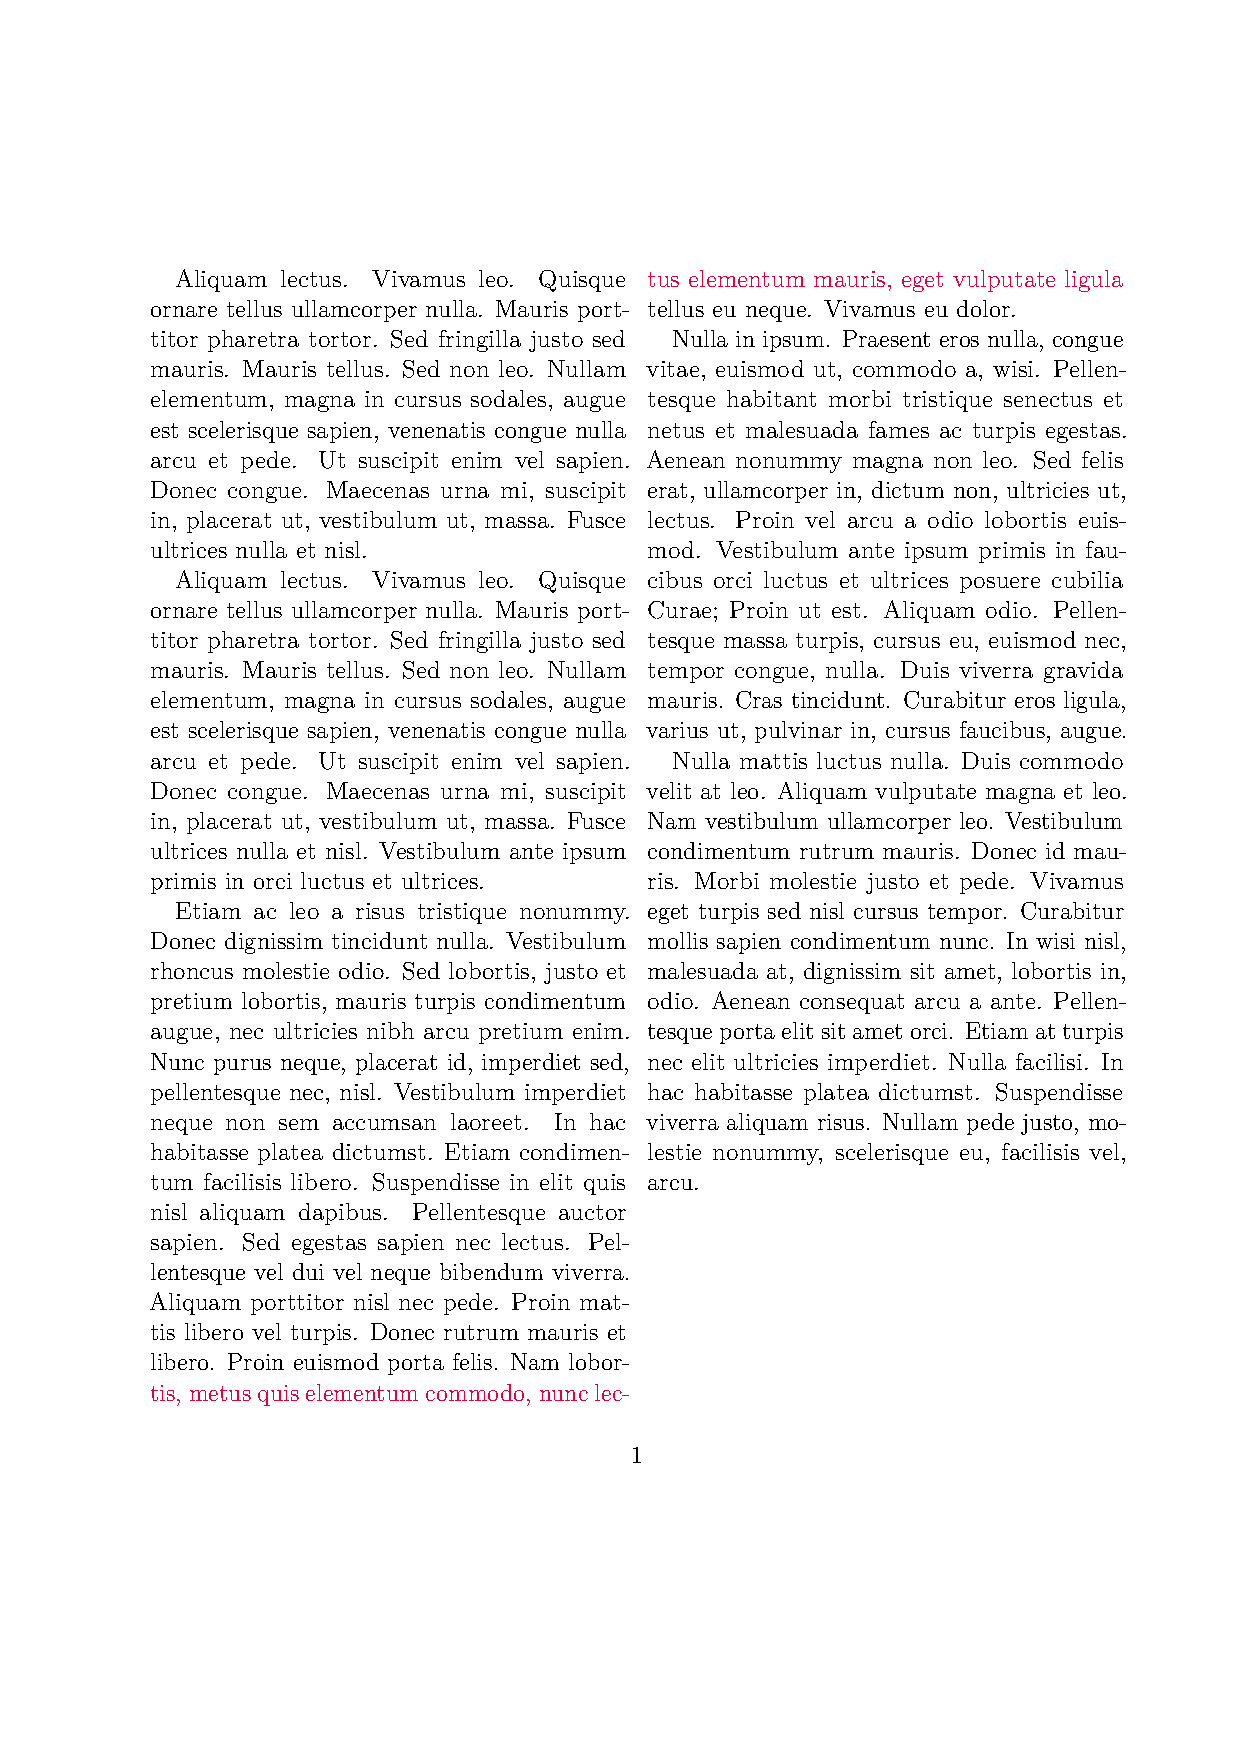
\includegraphics[width=\textwidth,page=1]{examples/widow.pdf}
  \end{center}
% \end{minipage}
\end{subfigure}
\hfill
\begin{subfigure}[t]{0.48\textwidth}
  \caption{Potlačený sirotek}
% \begin{minipage}{5cm}
  \begin{center}
    \includegraphics[width=\textwidth,page=2]{examples/widow.pdf}
  \end{center}
% \end{minipage}
\end{subfigure}
\caption{Příklad potlačení sirotků}
\label{fig:sirotek}
\end{figure}

% \subsubsection{Možnosti nastavení}

Balíček \balicek{Lua-widow-control} lze nastavit pomocí několika voleb. Ty je možné zadat jako čárkou oddělené volby 
v příkazu  \verb|\usepackage[<volby>]{lua-widow-control}|, nebo pomocí příkazu 
\verb|\lwcsetup{<volby>}|.

Následující volby umožňují změnit metodu použitou pro zamezení parchantů:

 \begin{description}
   \item[default] – nepřidává žádné vertikální mezery, používá pouze prodloužení odstavců. Tato metoda by měla odstranit 95 \% parchantů, může ovšem vést k příliš vzdušným odstavcům.
   \item[strict] – přísnější nastavení, které dbá, aby změny zalomení odstavců byly co nejméně postřehnutelné.  Odstraní ovšem pouze třetinu parchantů.
   \item[balanced] – nejdříve přidává vertikální mezery, pokud to nestačí, prodlouží odstavce. Tato metoda odstraní až 90 \% parchantů.
  \end{description}




\subsection{Balíček \balicek{Luavlna}}

Podle českých a slovenských typografických zvyklostí by se na koncích řádků neměly vyskytovat jednopísmenné předložky nebo spojky. 
Tomu se dá v \TeX u zabránit vložením znaku \verb|~| mezi předložku a následující slovo. Pro zjednodušení této činnosti existuje
několik nástrojů, například program \balicek{Vlna} Petra Olšáka, nebo balíček \balicek{Encxvlna} vytvořený také Petrem Olšákem a Zdeňkem Wagnerem.

Balíček \balicek{Luavlna} \cite{luavlna} využívá možnosti Lua\TeX u pro úpravu plně zpracovaných nódů textu před zalomením do odstavců. 
V tomto stádiu jsou již všechna makra expandována, takže nezlomitelná mezera může být snadno vložena na všechna místa, kde by se měla nacházet.

\balicek{Luavlna} zamezuje zalomení řádků v následujících situacích:

\begin{itemize}
  \item za jednoslovnými předložkami
  \item u iniciál
  \item u akademických titulů
  \item mezi čísly a jednotkami
\end{itemize}
  

\begin{figure}
  \begin{minipage}{3in}

    \preventsingledebugon

    Text s krátkými souhláskami a samohláskami i dalšími jevy
    z nabídky možností (v textu možnými).

    Co třeba í znaky š diakritikou?

    Různé možnosti [v závorkách \textless i jiných znacích

    Podpora iniciál a titulů: M. J. Hegel, Ing. Běháková, Ph.D., Ž. Zíbrt,
    Ch. Borner.

    Podpora jednotek: 100,5 MN\cdot{}s, 100.5 kJ, 200 µA, $-1$ dag, 1 MB. 1 kJ.

    Uvnitř matematiky by mělo být zpracování vypnuté: $k \in \mathbb N$.

    \preventsingledebugoff
  \end{minipage}
  \caption{Ukázka užití balíčku Luavlna}
  \label{fig:luavlna}
\end{figure}

Ukázku použití balíčku můžete vidět na obrázku \ref{fig:luavlna}. Nezlomitelné
mezery jsou zvýrazněné růžově, díky použití volby \texttt{debug}. Balíček
nabízí řadu dalších voleb, například pro zakázání vkládání nezlomitelných 
mezer v určitých situacích:

\begin{description}
  \item [noprocess] – nespouštět zpracování dokumentu automaticky
  \item [noinitials] – nezpracovávat iniciály
  \item [nounits] – nezpracovávat SI jednotky
  \item [nopredegrees] – nezpracovávat tituly před jménem
  \item [nosufdegrees] – nezpracovávat tituly za jménem
\end{description}

Nastavení jednotlivých jazyků se provádí pomocí těchto příkazů\balicek{Luavlna} také poskytuje příkaz

  \begin{itemize}
    \item\verb|\singlechars{jazyk}{písmena}| – seznam písmen, u kterých se potlačuje zalamování řádků.

    \item\verb|\enablesplithyphens{jazyk}| –  nastaví podporu zalamování spojovníků pro daný jazyk.
    \item\verb|\preventsinglelang{jazyk}| – nastaví pravidla pro daný jazyk pro celý dokument.
  \end{itemize}

Jazyk lze  vybrat pomocí balíčků \balicek{Babel} nebo \balicek{Polyglossia}. Následující příklad
ukazuje, že v českém textu se vloží nezlomitelná mezera, po změně jazyka na angličtinu pomocí
\verb|\selectlanguage{english}| se zpracování mezer vypne. 
  


\begin{verbatim}
Příklad v češtině
\selectlanguage{english}
A thing.
\end{verbatim}

\preventsingledebugon

\noindent \fbox{A příklad česky.
\selectlanguage{english}
A something.}

\preventsingledebugoff

\selectlanguage{czech}


\bigskip

Zpracování celého dokumentu podle českých pravidel, bez ohledu na aktuálně zvolený jazyk, lze dosáhnout pomocí příkazu 
\verb|\preventsinglelang{czech}|.

\subsection{Balíček \balicek{Linebreaker}}

\newcommand\testbox[1]{%
  \parbox{120pt}{%
    \parindent=15pt%
    \tolerance=1%
    \pretolerance=1%
    #1
  }%
}


\newcommand\printtest[1]{%
  \linebreakerdisable%
  \begin{subfigure}{.45\textwidth}
    \centering
  \caption{Bez Linebreakeru}
  \noindent\testbox{%
    #1
  }%
  \end{subfigure}
  \linebreakerenable%
  \hfill%
  \begin{subfigure}{.45\textwidth}
    \centering
  \caption{S Linebreakerem}
  \testbox{%
    #1
  }%
  \end{subfigure}
}

Balíček \balicek{Linebreaker} \cite{linebreaker} brání přetečení textu boxů a odstavců. 
Příklad jeho použití můžete vidět na obrázku \ref{fig:linebreaker}, kde zamezí přetečení 
několika řádků při sazbě do úzkého sloupce. 

\balicek{Linebreaker} využívá callback Lua\TeX u pro zalomení odstavců, kde nahrazuje výchozí 
funkci pro zalomení upravenou verzí, která detekuje přetečení nebo podtečení lámaného 
textu. Při detekci tohoto problému, jej sází znovu s většími hodnotami
\verb|\tolerance| a \verb|\emergencystretch|, dokud se přetečení nepotlačí, nebo dokud se nedosáhne 
maximální hranice \verb|\tolerance|.

Výhodou je, že tyto změny \verb|\tolerance| a \verb|\emergencystretch| jsou lokální pouze 
pro aktuálně lámaný odstavec, zbytek textu nijak neovlivní. 


\begin{figure}
  \printtest{
    The example document given below creates two pages by using Lua code alone. You
will learn how to access TeX's boxes and counters from the Lua side, shipout a
page into the PDF file, create horizontal and vertical boxes (hbox and vbox),
create new nodes and manipulate the nodes links structure. 
  }
  \caption{Příklad využití balíčku \balicek{Linebreaker}}
  \label{fig:linebreaker}
\end{figure}

  % \subsubsection{Nastavení}

\balicek{Linebreaker} můžeme konfigurovat pomocí příkazu \verb|\linebreakersetup|:
  \begin{description}
    \item[maxcycles] – počet pokusů o přesázení odstavce
    \item[maxemergencystretch] – maximální hodnota \verb|\emergencystretch|
    \item[maxtolerance] – maximální hodnota \verb|tolerance|
  \end{description}

\begin{verbatim}
\linebreakersetup{
maxtolerance = 90,         % default 9999
maxemergencystretch = 1em, % default 3em
maxcycles = 4              % default 30
}
\end{verbatim}

\printbibliography

\begin{summary}
  This article focuses on the use of responsive design techniques to display
  web pages on devices with different display sizes, such as mobile phones,
  tablets, large monitors and printers. These methods allow optimizing the
  readability of a document on all devices by using different font sizes,
  individual page elements, and margins.

  We present how similar functionality can be achieved using \LaTeX.
  Specifically, it focuses on the use of Lua\LaTeX{} for automated typesetting,
  using packages \balicek{Responsive} for setting font size and line spacing according to page size,
  \balicek{Luavlna} to prevent the occurrence of
  single-letter prepositions at line breaks, \balicek{Lua-widow-control} to
  reduce orphan lines at page breaks and page starts, and \balicek{Linebreaker}
  to prevent line overflow.

  With these methods, a single source document can be used for different
  outputs, such as print versions, e-book readers, and web pages, and achieve
  optimal document display on all devices.

\keywords: automatic typesetting, responsive design, Lua\LaTeX
\end{summary}
\end{document}
